%%%%%%%%%%%%%%%%%%%%%%%%%%%%%%%%%%%%%%%%%%%%%%%%%%%%%%%%%%%%%%%%%%%%%%%%%%%%%%%%%%%%%%%%%%%%%%%%%%%%%%%%%%%%%%%%%%%%%%%%%%%%%%%%%%%%%%%%%%%%%%%%%%%%%%%%%%%%%%%%%%%
% Written By Michael Brodskiy
% Class: Electricity & Magnetism
% Professor: D. Wood
%%%%%%%%%%%%%%%%%%%%%%%%%%%%%%%%%%%%%%%%%%%%%%%%%%%%%%%%%%%%%%%%%%%%%%%%%%%%%%%%%%%%%%%%%%%%%%%%%%%%%%%%%%%%%%%%%%%%%%%%%%%%%%%%%%%%%%%%%%%%%%%%%%%%%%%%%%%%%%%%%%%

\include{Includes.tex}

\title{Homework 10}
\date{December 6, 2023}
\author{Michael Brodskiy\\ \small Professor: D. Wood}

\begin{document}

\maketitle

\begin{enumerate}

  \item As a simplified model of a planet being bombarded with cosmic rays at the poles, consider a conducting sphere of radius $R$ that is being charged with wires at the north and south poles that each have a current $I/2$ flowing onto the sphere, so that the total charge of the sphere is increasing with time $\left( \frac{dQ}{dt}=I \right)$.  Assume the charge is always distributed uniformly on the surface of the sphere.

    \begin{enumerate}

      \item Calculate the displacement current density just above the surface of the sphere.

    We can begin by finding a relationship between displacement current and the electric displacement:

    $$\vec{J}=\frac{\partial \vec{D}}{\partial t}\to\varepsilon_o\frac{\partial\vec{E}}{\partial t}$$

    We know the formula for the electric field to be:

    $$\vec{E}=\frac{Q}{4\pi\varepsilon_o R^2}\bold{\hat{r}}$$

    Thus, we may conclude:

    $$\vec{J}=\frac{\varepsilon_o}{4\pi\varepsilon_o R^2}\left( \frac{\partial Q}{\partial t} \right)$$
    $$\boxed{\vec{J}=\frac{I}{4\pi R^2}\bold{\hat{r}}}$$

      \item Use the Amp\`re-Maxwell equation to calculate the induced magnetic field just above the surface at location that is an angle $\theta$ from the north pole (latitude = $90^{\circ}-\theta$). [Hint: Use a ring of constant latitude as the amperian loop and use a cap-shaped enclosed surface of the loop that follows the surface of the sphere. Be sure to include both the physical current and the displacement current.]  (While this is an interesting calculation, note that this is not a significant contribution to the Earth’s magnetic field.)

        We may begin by expressing the equation as:

        $$\int \vec{B}\cdot d\vec{l}=\mu_o\left( \sum I \right)$$
        $$\vec{B}\int d\vec{l}=\mu_o\left( I+I_d \right)$$

        The situation can be sketched as follows:

        \begin{figure}[h]
          \centering
          \tikzset{every picture/.style={line width=0.75pt}} %set default line width to 0.75pt        

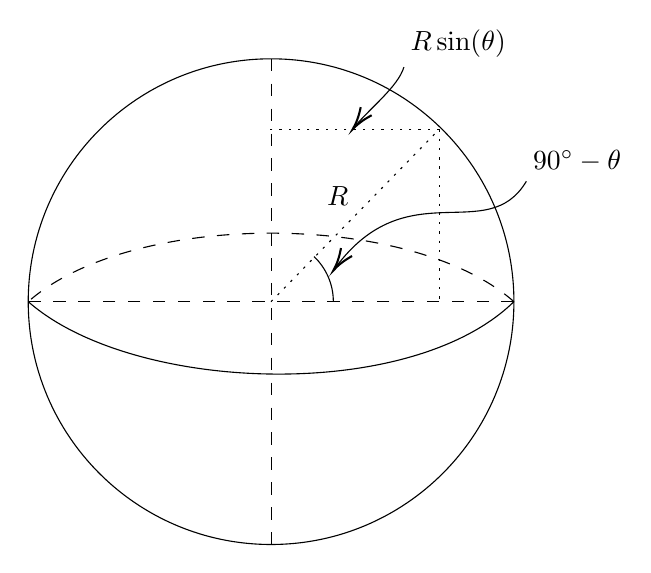
\begin{tikzpicture}[x=0.75pt,y=0.75pt,yscale=-1,xscale=1]
%uncomment if require: \path (0,485); %set diagram left start at 0, and has height of 485

%Shape: Circle [id:dp4936381296702055] 
\draw   (179,157) .. controls (179,92.38) and (231.38,40) .. (296,40) .. controls (360.62,40) and (413,92.38) .. (413,157) .. controls (413,221.62) and (360.62,274) .. (296,274) .. controls (231.38,274) and (179,221.62) .. (179,157) -- cycle ;
%Curve Lines [id:da7684497988482555] 
\draw    (179,157) .. controls (229,201) and (363,206) .. (413,157) ;
%Curve Lines [id:da031906274558686665] 
\draw  [dash pattern={on 4.5pt off 4.5pt}]  (413,157) .. controls (363,113) and (229,113) .. (179,157) ;
%Straight Lines [id:da7237618188990222] 
\draw  [dash pattern={on 4.5pt off 4.5pt}]  (296,40) -- (296,274) ;
%Straight Lines [id:da6805862140011472] 
\draw  [dash pattern={on 4.5pt off 4.5pt}]  (413,157) -- (179,157) ;
%Straight Lines [id:da6636715436204372] 
\draw  [dash pattern={on 0.84pt off 2.51pt}]  (296,157) -- (377,74) ;
%Shape: Arc [id:dp03958996945390081] 
\draw  [draw opacity=0] (316.72,135.3) .. controls (322.44,140.76) and (326,148.47) .. (326,157) -- (296,157) -- cycle ; \draw   (316.72,135.3) .. controls (322.44,140.76) and (326,148.47) .. (326,157) ;  
%Curve Lines [id:da7315028520131872] 
\draw    (419,99) .. controls (400.19,130.68) and (361.78,93.75) .. (327.05,140.56) ;
\draw [shift={(326,142)}, rotate = 305.54] [color={rgb, 255:red, 0; green, 0; blue, 0 }  ][line width=0.75]    (10.93,-3.29) .. controls (6.95,-1.4) and (3.31,-0.3) .. (0,0) .. controls (3.31,0.3) and (6.95,1.4) .. (10.93,3.29)   ;
%Straight Lines [id:da960505724523711] 
\draw  [dash pattern={on 0.84pt off 2.51pt}]  (377,74) -- (377,157.42) ;
%Straight Lines [id:da7630353719230638] 
\draw  [dash pattern={on 0.84pt off 2.51pt}]  (377,74) -- (293.58,74) ;
%Curve Lines [id:da15200728730904722] 
\draw    (360,44) .. controls (357.17,53.45) and (343.61,63.79) .. (336.47,72.5) ;
\draw [shift={(335.29,74)}, rotate = 306.71] [color={rgb, 255:red, 0; green, 0; blue, 0 }  ][line width=0.75]    (10.93,-3.29) .. controls (6.95,-1.4) and (3.31,-0.3) .. (0,0) .. controls (3.31,0.3) and (6.95,1.4) .. (10.93,3.29)   ;

% Text Node
\draw (421,95.6) node [anchor=south west] [inner sep=0.75pt]    {$90^{\circ } -\theta $};
% Text Node
\draw (334.5,112.1) node [anchor=south east] [inner sep=0.75pt]    {$R$};
% Text Node
\draw (362,40.6) node [anchor=south west] [inner sep=0.75pt]    {$R\sin( \theta )$};


\end{tikzpicture}

          \caption{The $90^{\circ}-\theta$ Shift Switches $\cos\to\sin$}
          \label{fig:1}
        \end{figure}

        We can then express the path as:

        $$\vec{B}(2\pi R\sin(\theta))=\mu_o\left(I+J\int_0^{2\pi}d\phi\int_0^\theta \sin(\theta)\,d\theta R^2\right)$$
        $$\vec{B}(2\pi R\sin(\theta))=\mu_o\left(I+\frac{I}{2}\left[ 1-\cos(\theta) \right]\right)$$

        And finally, we get:

        $$\boxed{\vec{B}=\frac{\mu_o I[3-\cos(\theta)]}{4\pi R\sin(\theta)}}$$

    \end{enumerate}

  \item Consider a capacitor with circular parallel plates of radius $a$ and separation $d$, where $d<<a$, there the capacitor is discharging with a current $I$.

    \begin{enumerate}

      \item Find the Poynting vector in the space between the plates. Assume that the surface charge is distributed uniformly over the plates.

        We may find the Poynting vector using the relation:

        $$\oint \vec{B}\cdot d\vec{A}=\mu_o\varepsilon_o\frac{d}{dt}\oint \vec{E}\cdot d\vec{A}$$

        Given the uniform charge contained within the area as $q$, we may find:

        $$\vec{E}=\frac{\sigma}{\varepsilon_o}$$
        $$\vec{E}=\frac{q}{\pi\varepsilon_o a^2}$$

        From here, we get:

        $$\vec{B}\oint d\vec{r}=\mu_o\varepsilon_o\frac{d}{dt}\left(\frac{q}{\pi\varepsilon_o a^2} \int d\vec{A}\right)$$
        $$\vec{B}(2\pi r)=\mu_o\varepsilon_o\frac{\pi r^2}{\pi\varepsilon_o a^2}\frac{dq}{dt}$$
        $$\vec{B}=\frac{\mu_or}{2\pi a^2}\frac{dq}{dt}$$

        The change in charge with respect to time may be described as the current, so we get:

        $$\vec{B}=\frac{\mu_orI}{2\pi a^2}$$

        We can then find the Poynting vector, using:

        $$\vec{S}=\frac{1}{\mu_o}\left( \vec{E}\cdot\vec{B} \right)\bold{\hat{r}}$$
        $$\vec{S}=\frac{1}{\mu_o}\left( \frac{q}{\pi\varepsilon_o a^2}\cdot\frac{\mu_orI}{2\pi a^2} \right)\bold{\hat{r}}$$

        This finally gives:

        $$\boxed{\vec{S}=\frac{qrI}{2\pi^2\varepsilon_o a^4}\bold{\hat{r}}}$$

      \item Calculate the rates of energy flow out of the volume between the plates by integrating $\vec{S}$ over an appropriate surface and show that it is equal to $|IV|$.

        The energy flow out of the volume may be defined as:

        $$P=\int \vec{S}\,dA$$
        $$P=\vec{S}(2\pi a d)$$

        Plugging in the value from (a) for $\vec{S}$, and evaluating at $r=a$ we get:

        $$P=\left( \frac{qaI}{2\pi^2\varepsilon_o a^4} \right)\left( 2\pi ad \right)$$
        $$P_{out}=\left( \frac{qId}{\pi\varepsilon_o a^2} \right)$$

        The flow out would be the negative equivalent:

        $$\boxed{P_{out}=\frac{qId}{\pi\varepsilon_o a^2}}$$

        We can see that the voltage may be defined as:

        $$V=\frac{qd}{\pi\varepsilon_o a^2}$$

        And that we then get the power outflow as:

        $$P=-IV=|-IV|$$

    \end{enumerate}

  \item An ideal parallel plate capacitor with area $A$ and separation $d$ is oriented with the lower plate in the $xy$ plane and is immersed in a uniform horizontal magnetic field $\vec{B}=B_o\bold{\hat{x}}$. The capacitor starts with a charge $+Q$ on the lower plate and $-Q$ on the upper plate. At time $t=0$, a vertical wire with resistance $R$ is connected between the plates.

    \begin{enumerate}

      \item Find the momentum (magnitude and direction) stored in the $\vec{E}$ and $\vec{B}$ fields at time $t=0$.

        The magnetic field is given as:

        $$\vec{B}=B_o\bold{\hat{x}}$$

        The electric field can be defined as:

        $$\vec{E}=\frac{Q}{\varepsilon_o A}\bold{\hat{z}}$$

        The momentum density is defined as:

        $$\frac{\vec{P}}{V}=\varepsilon_o\vec{E}\times\vec{B}$$

        With $V=Ad$, we get:

        $$\vec{P}=\varepsilon_oAd\left(\vec{E}\times\vec{B}\right)$$
        $$\vec{P}=\varepsilon_oAd\left(\frac{Q}{\varepsilon_o A}\bold{\hat{z}}\times B_o\bold{\hat{x}}\right)$$
        $$\vec{P}=\varepsilon_oAd\left|\begin{matrix} \bold{\hat{x}} & \bold{\hat{y}} & \bold{\hat{z}}\\ 0 & 0 & \frac{Q}{\varepsilon_o A}\\ B_o & 0 & 0\\ \end{matrix}\right|$$

        Evaluating the matrix, we get:

        $$\vec{P}=\varepsilon_oAd\left( \frac{B_oQ}{\varepsilon_o A} \right)\bold{\hat{y}}$$
        $$\boxed{\vec{P}=dB_oQ\bold{\hat{y}}}$$

      \item Find the force on the wire as a function of time

        We know that the voltage across the capacitor may be expressed as:

        $$V=\frac{q}{C}$$

        With this scenario, we may express the voltage as:

        $$IR=\frac{q}{C}$$

        The current may be expressed as:

        $$-R\frac{dq}{dt}=\frac{q}{C}$$

        Rearranging the expression, we get:

        $$\frac{dq}{q}=-\frac{1}{RC}\,dt$$

        This yields the solution:

        $$\ln(q)=-\frac{t}{RC}+c$$

        We know that, at time $t=0$, $q=Q$, which gives us:

        $$c=\ln(Q)$$

        Thus, we may write:

        $$q=Qe^{-\frac{t}{RC}}$$

        From here, we may take the derivative with respect to time to discover:

        $$I=-\frac{Q}{RC}e^{-\frac{t}{RC}}$$

        The force on the wire may be expressed as:

        $$\vec{F}=I\,d\vec{l}\times\vec{B},\quad d\vec{l}\to d\bold{\hat{z}}\text{\footnote{Note: $d$ here is the distance, not a differential}}$$

        This gives us:

        $$\vec{F}=Id\bold{\hat{z}}\times B_o\bold{\hat{x}}$$
        $$\vec{F}=\frac{Qd}{RC}e^{-\frac{t}{RC}}\bold{\hat{z}}\times B_o\bold{\hat{x}}$$
        $$\vec{F}=\left|\begin{matrix} \bold{\hat{x}} & \bold{\hat{y}} & \bold{\hat{z}}\\ 0 & 0 & Id\\ B_o & 0 & 0\\ \end{matrix}\right|$$

        Finally, we get:

        $$\boxed{\vec{F}=\frac{QdB_o}{RC}e^{-\frac{t}{RC}}\bold{\hat{y}}}$$

      \item Find the total impulse $\left( \int\vec{F}\,dt \right)$ on the wire for $t\to\infty$. Compare this with the change in stored momentum.

        The impulse may be defined as:

        $$\vec{j}=\int_0^\infty \frac{QdB_o}{RC}e^{-\frac{t}{RC}}\bold{\hat{y}}\,dt$$

        The $(RC)^{-1}$ coefficient cancels out, leaving us with:

        $$\boxed{\vec{j}=QdB_o\bold{\hat{y}}}$$

        As calculated above, the initial momentum is:

        $$\vec{P}=QdB_o\bold{\hat{y}}$$

        Given infinite time, the momentum will deplete until it is zero, giving us:

        $$\Delta\vec{P}=-QdB_o\bold{\hat{y}}$$

        Thus, the total impulse is equal in magnitude but opposite in direction to the change in the momentum field vector.

    \end{enumerate}

  \item We re-revisit the spinning hollow sphere from earlier assignments — a hollow insulating sphere of radius $R$ and mass $M$ centered at the origin is covered with a uniform surface charge $\sigma=Q/(4\pi R^2)$, rotating about the $z$-axis with angular frequency $\omega$. This time we consider both the magnetic field and the electric field produced by the sphere itself.

    \begin{enumerate}

      \item Calculate the total energy of the electric and magnetic fields. You can use the results from Homework 8, Problem 1 for the $\vec{B}$-field — you do not need to re-derive it.  Be sure to include the magnetic field inside the sphere as well as outside.

        We know that the energy density may be written as:

        $$\mathcal{U}=\frac{\varepsilon_o}{2}\vec{E}^2+\frac{1}{2\mu_o}\vec{B}^2$$

        We can decompose the energy into components to get:

        $$\mathcal{U}=\mathcal{U}_{\vec{E},in}+\mathcal{U}_{\vec{E},out}+\mathcal{U}_{\vec{B},in}+\mathcal{U}_{\vec{B},out}$$

        We know that we may define the electric field as:

        $$\vec{E}_{out}=\frac{Q}{4\pi\varepsilon_o r^2}\bold{\hat{r}}$$
        $$\vec{E}_{in}=0$$

        From Homework 8, Problem 1, the magnetic field may be defined as:

        $$\vec{B}=\frac{\mu_o\sigma\omega R^4}{3r^3}\left[ 2\cos(\theta)\bold{\hat{r}}+\sin(\theta)\hat{\theta} \right]$$

        We know that, inside, $\theta=0$ and $r\to R$, which gives us:

        $$\vec{B}_{out}=\frac{\mu_o\sigma\omega R^4}{3r^3}\left[ 2\cos(\theta)\bold{\hat{r}}+\sin(\theta)\hat{\theta} \right]$$
        $$\vec{B}_{in}=\frac{2}{3}\mu_o\sigma\omega R\bold{\hat{r}}$$

        We can define two energies that are easier for us to calculate as:

        $$\mathcal{U}_{\vec{E},in}=0$$

        And then:

        $$\mathcal{U}_{\vec{B},in}=\frac{1}{2\mu_o}\left( \frac{2}{3}\mu_o\sigma\omega R \right)^2$$
        $$\mathcal{U}_{\vec{B},in}=\frac{2}{9}\mu_o\sigma^2\omega^2 R^2$$
        $$\mathcal{U}_{\vec{B},in}=\frac{2}{9}\mu_o\omega^2 R^2\cdot\frac{Q^2}{16\pi^2R^4}$$
        $$\mathcal{U}_{\vec{B},in}=\frac{\mu_o\omega^2Q^2}{72\pi^2R^2}$$

        We then multiply by the volume to get:

        $$U_{\vec{B},in}=\frac{\mu_o\omega^2Q^2}{72\pi^2R^2}\left( \frac{4}{3}\pi R^3 \right)$$
        $$U_{\vec{B},in}=\frac{\mu_o\omega^2Q^2R}{54\pi}$$

        For the outer regions we now find:

        $$\mathcal{U}_{\vec{E},out}=\frac{\varepsilon_o}{2}\left( \frac{Q}{4\pi\varepsilon_o R^2} \right)^2$$
        $$\mathcal{U}_{\vec{E},out}=\frac{\varepsilon_o}{2}\left( \frac{Q^2}{16\pi^2\varepsilon_o^2 R^4} \right)$$
        $$\mathcal{U}_{\vec{E},out}=\frac{Q^2}{32\pi^2\varepsilon_o R^4}$$

        We now calculate the energy:

        $$U_{\vec{E},out}=\frac{Q^2}{32\pi^2\varepsilon_o}\int_0^{2\pi}\,d\phi\int_0^\pi\sin(\theta)\,d\theta\int_{R}^\infty \frac{1}{r^2}\,dr$$
        $$U_{\vec{E},out}=\frac{Q^2}{8\pi\varepsilon_oR}$$

        Returning to the outer fields, we find the magnetic energy density:

        $$\mathcal{U}_{\vec{B},out}=\frac{1}{2\mu_o}\left(\frac{\mu_o\sigma\omega R^4}{3r^3}\left[ 2\cos(\theta)\bold{\hat{r}}+\sin(\theta)\hat{\theta} \right]  \right)^2$$
        $$\mathcal{U}_{\vec{B},out}=\frac{1}{2\mu_o}\left(\frac{\mu_o^2\sigma^2\omega^2 R^8}{9r^6}\left[ 4\cos^2(\theta)+\sin^2(\theta)\right]  \right)$$
        $$\mathcal{U}_{\vec{B},out}=\frac{\mu_o\sigma^2\omega^2 R^8}{18r^6}\left[ 4\cos^2(\theta)+\sin^2(\theta)\right] $$
        $$\mathcal{U}_{\vec{B},out}=\frac{\mu_oQ^2\omega^2 R^4}{288\pi^2r^6}\left[ 4\cos^2(\theta)+\sin^2(\theta)\right] $$

        Once again, we find the energy:

        $$U_{\vec{B},out}=\frac{\mu_oQ^2\omega^2 R^4}{288\pi^2}\int_0^{2\pi}\,d\phi\underbrace{\int_0^\pi\left[ 4\cos^2(\theta)\sin(\theta)+\sin^3(\theta)\right]\,d\theta}_{4}\underbrace{\int_R^\infty \frac{1}{r^4}\,dr}_{\frac{1}{3R^3}}$$
        $$U_{\vec{B},out}=\frac{\mu_oQ^2\omega^2 R}{108\pi}$$

        We sum all of the energy components to get:

        $$U_{tot}=U_{\vec{E},in}+U_{\vec{E},out}+U_{\vec{B},in}+U_{\vec{B},out}$$
        $$U_{tot}=0+\frac{Q^2}{8\pi\varepsilon_o R}+\frac{\mu_o\omega^2Q^2R}{54\pi}+\frac{\mu_oQ^2\omega^2 R}{108\pi}$$

        Thus, we finally get:

        $$\boxed{U_{tot}=\frac{Q^2}{8\pi\varepsilon_o R}+\frac{\mu_o\omega^2Q^2R}{36\pi}}$$

      \item Calculate the total angular momentum of the electromagnetic fields, $L_Q$.

        To find the angular momentum, we must find $\vec{g}$. We can first say:

        $$\vec{g}_{in}=0$$

        since $\vec{E}_{in}=0$. To find $\vec{g}_{out}$, we can use:

        $$\vec{g}=\varepsilon_o\vec{E}\times\vec{B}$$

        This gives us:

        $$\vec{g}_{out}=\varepsilon_o\left(\frac{Q}{4\pi\varepsilon_o r^2}\right)\left( \frac{\mu_o\sigma\omega R^4}{3r^3} \right)\left[ \cancel{\bold{\hat{r}}\times 2\cos(\theta)\bold{\hat{r}}}+\bold{\hat{r}}\times\sin(\theta)\hat{\theta} \right]$$
        $$\vec{g}_{out}=\varepsilon_o\left(\frac{Q}{4\pi\varepsilon_o r^2}\right)\left( \frac{\mu_o\sigma\omega R^4}{3r^3} \right)\left[ \bold{\hat{r}}\times\sin(\theta)\hat{\theta} \right]$$
        $$\vec{g}_{out}=\frac{\mu_oQ\sigma\omega R^4}{12\pi r^5}\sin(\theta)\hat{\phi}$$

        We can then find the angular momentum according to:

        $$\vec{l}=\vec{r}\times\vec{g}$$
        $$\vec{l}=r\left( \frac{\mu_oQ\sigma\omega R^4}{12\pi r^5}\sin(\theta) \right)[\bold{\hat{r}}\times\hat{\phi}]$$
        $$\vec{l}=-\frac{\mu_oQ\sigma\omega R^4}{12\pi r^4}\sin(\theta)\hat{\theta}$$

        We know that, due to the sphere spinning along the $z$-axis, only angular momentum along the $z$ component will contribute. Thus, we get:

        $$\vec{l}_z=-\frac{\mu_oQ\sigma\omega R^4}{12\pi r^4}\sin(\theta)(\hat{\theta}\cdot\bold{\hat{z}}$$
        $$\vec{l}_z=\frac{\mu_oQ\sigma\omega R^4}{12\pi r^4}\sin^2(\theta)$$

        To find $L_Q$, we may write:

        $$L_Q=\oint \vec{l}\,d\tau$$

        This gives us:

        $$\vec{L}_Q=\frac{\mu_oQ^2\omega R^2}{48\pi^2}\int_0^{2\pi}\,d\phi\int_0^{\pi}\sin^3(\theta)\,d\theta\int_R^\infty \frac{1}{r^2}\,dr$$
        $$\boxed{\vec{L}_Q=\frac{\mu_oQ^2\omega R}{18\pi}\bold{\hat{z}}}$$

      \item Consider a spinning shell whose rest energy $(Mc^2)$ is equal to its electrostatic potential energy $(Q^2/(8\pi\varepsilon_o R))$. Find the ratio between the mechanical ($L_M$) and electromagnetic ($L_Q$) contributions to the angular momentum. Use the fact that $c=1/\sqrt{\varepsilon_o\mu_o}$.

        Given this, we can set:

        $$\vec{L}_Q\Rightarrow\frac{\mu_oQ^2\omega R}{18\pi}=\frac{Q^2}{8\pi\varepsilon_o R}$$

        We can rearrange to get:

        $$\vec{L}_Q=(Mc^2)\frac{4c^2\mu_o\varepsilon_o\omega R^2}{9}$$

        We know that:

        $$c^2=\frac{1}{\mu_o\varepsilon_o}$$

        This gives us:

        $$\vec{L}_Q=\frac{4M\omega R^2}{9}\bold{\hat{z}}$$

        For a spinning shell with mass $M$, we may write:

        $$I=\frac{2}{3}MR^2$$

        We also know:

        $$\vec{L}_M=I\vec{\omega}$$

        This gives:

        $$\vec{L}_M=\frac{2}{3}M\omega R^2\bold{\hat{z}}$$

        Finding the ratio, we get:

        $$\boxed{\frac{\vec{L}_M}{\vec{L}_Q}=\frac{(2)(9)M\omega R^2\bold{\hat{z}}}{(3)(4)M\omega R^2\bold{\hat{z}}}=\frac{3}{2}}$$

    \end{enumerate}

\end{enumerate}

\end{document}

